\chapterimage{media/headerLogo.png}
\section{Verwendete Software}
\label{sec:used-software}

\vspace{3cm}

\begin{savenotes}
    \begin{table}[!ht]
    \centering
        \begin{tabular}{lll}
        \rowcolor[HTML]{FFFFFF} 
        \textbf{Software} & \textbf{Kategorie} & \textbf{Version} \\ \hline
        \rowcolor[HTML]{FFFFFF} 
        Python & Programmiersprache & 3.8.3\\
        \rowcolor[HTML]{EFEFEF} 
        pdfminer.six\footnote{Webseite: \url{https://pypi.org/project/pdfminer.six/}} & Informationsextraktion & 20200517\\
        \rowcolor[HTML]{FFFFFF}
        pyLDAviz\footnote{Github: \url{https://github.com/bmabey/pyLDAvis}} & Themenmodellierung & 2.1.2\\
        \rowcolor[HTML]{EFEFEF} 
        Gensim\footnote{Webseite: \url{https://radimrehurek.com/gensim}} & Themenmodellierung & 3.8.3\\
        \rowcolor[HTML]{FFFFFF} 
        spaCy\footnote{Github: \url{https://github.com/explosion/spaCy}} & NLP & 2.2.4\\
        \rowcolor[HTML]{EFEFEF} 
        scikit-learn\footnote{Webseite: \url{https://scikit-learn.org}} & Maschinelles Lernen & 0.23.1\\
        Jupyter Lab\footnote{Webseite: \url{https://jupyter.org}} & IDE & 2.1.4\\
        \rowcolor[HTML]{EFEFEF} 
        pandas\footnote{Webseite: \url{https://pandas.pydata.org}} & Datenverwaltung & 1.0.4\\
        \rowcolor[HTML]{FFFFFF} 
        NumPy\footnote{Webseite: \url{https://numpy.org}} & wissenschaftliches Rechnen & 1.18.4\\

        \end{tabular}%
    \caption{Übersicht der verwendeten Software}
    \label{tab:used-software}
    \end{table}
\end{savenotes}

\clearpage

\section{Konfusionsmatrizen der externen Pflichtenhefte}
\label{app:pflichtenhefte}

\vspace{2cm}

%%%%%%%%%%%
%%%% PH_A01
\begin{table}[!ht]
    \begin{subtable}{0.465\textwidth}
    \centering
        \resizebox{0.60\textwidth}{!}{%
        \begin{tabular}{cc|cc}
            \multicolumn{1}{c}{} &\multicolumn{1}{c}{} &\multicolumn{2}{c}{\scriptsize Vorhergesagt} \\ 
            \multicolumn{1}{c}{} & 
            \multicolumn{1}{c|}{} & 
            \multicolumn{1}{c}{Wahr} & 
            \multicolumn{1}{c}{Falsch} \\ \hline
            \multirow[c]{2}{*}{\rotatebox[origin=tr]{90}{\tiny Tatsächlich}}
            & Wahr      & 109    & 65     \\ [1.5ex]
            & Falsch    & 36    & 24    \\ \hline
        \end{tabular}
        }
        \caption{SAFE Confusion Matrix}
        \label{cmA01safe}
    \end{subtable}
    \hspace{0.2cm}
    \begin{subtable}{0.465\textwidth}
    \centering
        \resizebox{0.60\textwidth}{!}{%
        \begin{tabular}{cc|cc}
            \multicolumn{1}{c}{} &\multicolumn{1}{c}{} &\multicolumn{2}{c}{\scriptsize Vorhergesagt} \\ 
            \multicolumn{1}{c}{} & 
            \multicolumn{1}{c|}{} & 
            \multicolumn{1}{c}{Wahr} & 
            \multicolumn{1}{c}{Falsch} \\ \hline
            \multirow[c]{2}{*}{\rotatebox[origin=tr]{90}{\tiny Tatsächlich}}
            & Wahr      & 118   & 56     \\ [1.5ex]
            & Falsch    & 22    & 38    \\ \hline
        \end{tabular}
        }
        \caption{thesis Confusion Matrix}
        \label{cmA01thesis}
    \end{subtable}
    \vspace{0.1cm}
    \begin{subtable}{0.465\textwidth}
    \centering
        \resizebox{\textwidth}{!}{%
        \begin{tabular}{
        >{\columncolor[HTML]{FFFFFF}}r 
        >{\columncolor[HTML]{FFFFFF}}r 
        >{\columncolor[HTML]{FFFFFF}}r 
        >{\columncolor[HTML]{FFFFFF}}r 
        >{\columncolor[HTML]{FFFFFF}}r }
        \multicolumn{1}{l}{\cellcolor[HTML]{FFFFFF}} &
          \multicolumn{1}{l}{\cellcolor[HTML]{FFFFFF}precision} &
          \multicolumn{1}{l}{\cellcolor[HTML]{FFFFFF}recall} &
          \multicolumn{1}{l}{\cellcolor[HTML]{FFFFFF}f1-score} &
          \multicolumn{1}{l}{\cellcolor[HTML]{FFFFFF}support} \\ \cline{2-5} 
        \multicolumn{1}{r|}{\cellcolor[HTML]{FFFFFF}}             &      &      &      & \multicolumn{1}{r|}{\cellcolor[HTML]{FFFFFF}}    \\ \cline{1-1}
        \multicolumn{1}{|r}{\cellcolor[HTML]{FFFFFF}0}            & 0.25 & 0.85 & 0.39 & \multicolumn{1}{r|}{\cellcolor[HTML]{FFFFFF}60}  \\ \hline
        \multicolumn{1}{|r}{\cellcolor[HTML]{FFFFFF}1}            & 0.73 & 0.14 & 0.23 & \multicolumn{1}{r|}{\cellcolor[HTML]{FFFFFF}174}  \\ \hline
                                                                  &      &      &      &                                                  \\ \hline
        \multicolumn{1}{|r}{\cellcolor[HTML]{FFFFFF}accuray}      &      &      & 0.32 & \multicolumn{1}{r|}{\cellcolor[HTML]{FFFFFF}234} \\
        \multicolumn{1}{|r}{\cellcolor[HTML]{FFFFFF}macro avg}    & 0.49 & 0.49 & 0.31 & \multicolumn{1}{r|}{\cellcolor[HTML]{FFFFFF}234} \\
        \multicolumn{1}{|r}{\cellcolor[HTML]{FFFFFF}weighted avg} & 0.61 & 0.32 & 0.27 & \multicolumn{1}{r|}{\cellcolor[HTML]{FFFFFF}234} \\ \hline
        \end{tabular}%
        }
        \caption{SAFE POS-Muster}
        \label{csA01safe}
    \end{subtable}
    \hspace{0.2cm}
    \begin{subtable}{0.465\textwidth}
    \centering
        \resizebox{\textwidth}{!}{%
        \begin{tabular}{
        >{\columncolor[HTML]{FFFFFF}}r 
        >{\columncolor[HTML]{FFFFFF}}r 
        >{\columncolor[HTML]{FFFFFF}}r 
        >{\columncolor[HTML]{FFFFFF}}r 
        >{\columncolor[HTML]{FFFFFF}}r }
        \multicolumn{1}{l}{\cellcolor[HTML]{FFFFFF}} &
          \multicolumn{1}{l}{\cellcolor[HTML]{FFFFFF}precision} &
          \multicolumn{1}{l}{\cellcolor[HTML]{FFFFFF}recall} &
          \multicolumn{1}{l}{\cellcolor[HTML]{FFFFFF}f1-score} &
          \multicolumn{1}{l}{\cellcolor[HTML]{FFFFFF}support} \\ \cline{2-5} 
        \multicolumn{1}{r|}{\cellcolor[HTML]{FFFFFF}}             &      &      &      & \multicolumn{1}{r|}{\cellcolor[HTML]{FFFFFF}}    \\ \cline{1-1}
        \multicolumn{1}{|r}{\cellcolor[HTML]{FFFFFF}0}            & 0.40 & 0.63 & 0.49 & \multicolumn{1}{r|}{\cellcolor[HTML]{FFFFFF}60}  \\ \hline
        \multicolumn{1}{|r}{\cellcolor[HTML]{FFFFFF}1}            & 0.84 & 0.68 & 0.75 & \multicolumn{1}{r|}{\cellcolor[HTML]{FFFFFF}174}  \\ \hline
                                                                  &      &      &      &                                                  \\ \hline
        \multicolumn{1}{|r}{\cellcolor[HTML]{FFFFFF}accuray}      &      &      & 0.67 & \multicolumn{1}{r|}{\cellcolor[HTML]{FFFFFF}234} \\
        \multicolumn{1}{|r}{\cellcolor[HTML]{FFFFFF}macro avg}    & 0.62 & 0.66 & 0.62 & \multicolumn{1}{r|}{\cellcolor[HTML]{FFFFFF}234} \\
        \multicolumn{1}{|r}{\cellcolor[HTML]{FFFFFF}weighted avg} & 0.73 & 0.67 & 0.69 & \multicolumn{1}{r|}{\cellcolor[HTML]{FFFFFF}234} \\ \hline
        \end{tabular}%
        }
        \caption{thesis POS-Muster}
        \label{csA01thesis}
    \end{subtable}%
    \caption{Konfusionsmatrizen und Kennzahlen des PH\_A01}
    \label{tabs:resultsPHA01}
\end{table}

\vspace{2cm}

%%%%%%%%%%%
%%%% PH_A02
\begin{table}[!ht]
    \begin{subtable}{0.465\textwidth}
    \centering
        \resizebox{0.60\textwidth}{!}{%
        \begin{tabular}{cc|cc}
            \multicolumn{1}{c}{} &\multicolumn{1}{c}{} &\multicolumn{2}{c}{\scriptsize Vorhergesagt} \\ 
            \multicolumn{1}{c}{} & 
            \multicolumn{1}{c|}{} & 
            \multicolumn{1}{c}{Wahr} & 
            \multicolumn{1}{c}{Falsch} \\ \hline
            \multirow[c]{2}{*}{\rotatebox[origin=tr]{90}{\tiny Tatsächlich}}
            & Wahr      & 48    & 40    \\ [1.5ex]
            & Falsch    & 37    & 18    \\ \hline
        \end{tabular}
        }
        \caption{SAFE Confusion Matrix}
        \label{cmA02safe}
    \end{subtable}
    \hspace{0.2cm}
    \begin{subtable}{0.465\textwidth}
    \centering
        \resizebox{0.60\textwidth}{!}{%
        \begin{tabular}{cc|cc}
            \multicolumn{1}{c}{} &\multicolumn{1}{c}{} &\multicolumn{2}{c}{\scriptsize Vorhergesagt} \\ 
            \multicolumn{1}{c}{} & 
            \multicolumn{1}{c|}{} & 
            \multicolumn{1}{c}{Wahr} & 
            \multicolumn{1}{c}{Falsch} \\ \hline
            \multirow[c]{2}{*}{\rotatebox[origin=tr]{90}{\tiny Tatsächlich}}
            & Wahr      & 62    & 26    \\ [1.5ex]
            & Falsch    & 23    & 32    \\ \hline
        \end{tabular}
        }
        \caption{thesis Confusion Matrix}
        \label{cmA02thesis}
    \end{subtable}
    \vspace{0.1cm}
    \begin{subtable}{0.465\textwidth}
    \centering
        \resizebox{\textwidth}{!}{%
        \begin{tabular}{
        >{\columncolor[HTML]{FFFFFF}}r 
        >{\columncolor[HTML]{FFFFFF}}r 
        >{\columncolor[HTML]{FFFFFF}}r 
        >{\columncolor[HTML]{FFFFFF}}r 
        >{\columncolor[HTML]{FFFFFF}}r }
        \multicolumn{1}{l}{\cellcolor[HTML]{FFFFFF}} &
          \multicolumn{1}{l}{\cellcolor[HTML]{FFFFFF}precision} &
          \multicolumn{1}{l}{\cellcolor[HTML]{FFFFFF}recall} &
          \multicolumn{1}{l}{\cellcolor[HTML]{FFFFFF}f1-score} &
          \multicolumn{1}{l}{\cellcolor[HTML]{FFFFFF}support} \\ \cline{2-5} 
        \multicolumn{1}{r|}{\cellcolor[HTML]{FFFFFF}}             &      &      &      & \multicolumn{1}{r|}{\cellcolor[HTML]{FFFFFF}}    \\ \cline{1-1}
        \multicolumn{1}{|r}{\cellcolor[HTML]{FFFFFF}0}            & 0.31 & 0.33 & 0.32 & \multicolumn{1}{r|}{\cellcolor[HTML]{FFFFFF}55}  \\ \hline
        \multicolumn{1}{|r}{\cellcolor[HTML]{FFFFFF}1}            & 0.56 & 0.55 & 0.55 & \multicolumn{1}{r|}{\cellcolor[HTML]{FFFFFF}88}  \\ \hline
                                                                  &      &      &      &                                                  \\ \hline
        \multicolumn{1}{|r}{\cellcolor[HTML]{FFFFFF}accuray}      &      &      & 0.46 & \multicolumn{1}{r|}{\cellcolor[HTML]{FFFFFF}144} \\
        \multicolumn{1}{|r}{\cellcolor[HTML]{FFFFFF}macro avg}    & 0.29 & 0.29 & 0.29 & \multicolumn{1}{r|}{\cellcolor[HTML]{FFFFFF}144} \\
        \multicolumn{1}{|r}{\cellcolor[HTML]{FFFFFF}weighted avg} & 0.46 & 0.46 & 0.46 & \multicolumn{1}{r|}{\cellcolor[HTML]{FFFFFF}144} \\ \hline
        \end{tabular}%
        }
        \caption{SAFE POS-Muster}
        \label{csA02safe}
    \end{subtable}%
    \hspace{0.2cm}
    \begin{subtable}{0.465\textwidth}
    \centering
        \resizebox{\textwidth}{!}{%
        \begin{tabular}{
        >{\columncolor[HTML]{FFFFFF}}r 
        >{\columncolor[HTML]{FFFFFF}}r 
        >{\columncolor[HTML]{FFFFFF}}r 
        >{\columncolor[HTML]{FFFFFF}}r 
        >{\columncolor[HTML]{FFFFFF}}r }
        \multicolumn{1}{l}{\cellcolor[HTML]{FFFFFF}} &
          \multicolumn{1}{l}{\cellcolor[HTML]{FFFFFF}precision} &
          \multicolumn{1}{l}{\cellcolor[HTML]{FFFFFF}recall} &
          \multicolumn{1}{l}{\cellcolor[HTML]{FFFFFF}f1-score} &
          \multicolumn{1}{l}{\cellcolor[HTML]{FFFFFF}support} \\ \cline{2-5} 
        \multicolumn{1}{r|}{\cellcolor[HTML]{FFFFFF}}             &      &      &      & \multicolumn{1}{r|}{\cellcolor[HTML]{FFFFFF}}    \\ \cline{1-1}
        \multicolumn{1}{|r}{\cellcolor[HTML]{FFFFFF}0}            & 0.54 & 0.58 & 0.56 & \multicolumn{1}{r|}{\cellcolor[HTML]{FFFFFF}55}  \\ \hline
        \multicolumn{1}{|r}{\cellcolor[HTML]{FFFFFF}1}            & 0.73 & 0.70 & 0.72 & \multicolumn{1}{r|}{\cellcolor[HTML]{FFFFFF}88}  \\ \hline
                                                                  &      &      &      &                                                  \\ \hline
        \multicolumn{1}{|r}{\cellcolor[HTML]{FFFFFF}accuray}      &      &      & 0.65 & \multicolumn{1}{r|}{\cellcolor[HTML]{FFFFFF}144} \\
        \multicolumn{1}{|r}{\cellcolor[HTML]{FFFFFF}macro avg}    & 0.42 & 0.43 & 0.43 & \multicolumn{1}{r|}{\cellcolor[HTML]{FFFFFF}144} \\
        \multicolumn{1}{|r}{\cellcolor[HTML]{FFFFFF}weighted avg} & 0.65 & 0.65 & 0.65 & \multicolumn{1}{r|}{\cellcolor[HTML]{FFFFFF}144} \\ \hline
        \end{tabular}%
        }
        \caption{thesis POS-Muster}
        \label{csA02thesis}
    \end{subtable}
    \caption{Konfusionsmatrizen und Kennzahlen des PH\_A02}
    \label{tabs:resultsPHA02}
\end{table}

%%%%%%%%%%%
%%%% PH_A03
\begin{table}[!ht]
    \begin{subtable}{0.465\textwidth}
    \centering
        \resizebox{0.60\textwidth}{!}{%
        \begin{tabular}{cc|cc}
            \multicolumn{1}{c}{} &\multicolumn{1}{c}{} &\multicolumn{2}{c}{\scriptsize Vorhergesagt} \\ 
            \multicolumn{1}{c}{} & 
            \multicolumn{1}{c|}{} & 
            \multicolumn{1}{c}{Wahr} & 
            \multicolumn{1}{c}{Falsch} \\ \hline
            \multirow[c]{2}{*}{\rotatebox[origin=tr]{90}{\tiny Tatsächlich}}
            & Wahr      & 153    & 102     \\ [1.5ex]
            & Falsch    & 108     & 139    \\ \hline
        \end{tabular}
        }
        \caption{SAFE Confusion Matrix}
        \label{cmA03safe}
    \end{subtable}
    \hspace{0.2cm}
    \begin{subtable}{0.465\textwidth}
    \centering
        \resizebox{0.60\textwidth}{!}{%
        \begin{tabular}{cc|cc}
            \multicolumn{1}{c}{} &\multicolumn{1}{c}{} &\multicolumn{2}{c}{\scriptsize Vorhergesagt} \\ 
            \multicolumn{1}{c}{} & 
            \multicolumn{1}{c|}{} & 
            \multicolumn{1}{c}{Wahr} & 
            \multicolumn{1}{c}{Falsch} \\ \hline
            \multirow[c]{2}{*}{\rotatebox[origin=tr]{90}{\tiny Tatsächlich}}
            & Wahr      & 202   & 53    \\ [1.5ex]
            & Falsch    & 81    & 166    \\ \hline
        \end{tabular}
        }
        \caption{thesis Confusion Matrix}
        \label{cmA03thesis}
    \end{subtable}
    \vspace{0.1cm}
    \begin{subtable}{0.465\textwidth}
    \centering
        \resizebox{\textwidth}{!}{%
        \begin{tabular}{
        >{\columncolor[HTML]{FFFFFF}}r 
        >{\columncolor[HTML]{FFFFFF}}r 
        >{\columncolor[HTML]{FFFFFF}}r 
        >{\columncolor[HTML]{FFFFFF}}r 
        >{\columncolor[HTML]{FFFFFF}}r }
        \multicolumn{1}{l}{\cellcolor[HTML]{FFFFFF}} &
          \multicolumn{1}{l}{\cellcolor[HTML]{FFFFFF}precision} &
          \multicolumn{1}{l}{\cellcolor[HTML]{FFFFFF}recall} &
          \multicolumn{1}{l}{\cellcolor[HTML]{FFFFFF}f1-score} &
          \multicolumn{1}{l}{\cellcolor[HTML]{FFFFFF}support} \\ \cline{2-5} 
        \multicolumn{1}{r|}{\cellcolor[HTML]{FFFFFF}}             &      &      &      & \multicolumn{1}{r|}{\cellcolor[HTML]{FFFFFF}}    \\ \cline{1-1}
        \multicolumn{1}{|r}{\cellcolor[HTML]{FFFFFF}0}            & 0.58 & 0.56 & 0.57 & \multicolumn{1}{r|}{\cellcolor[HTML]{FFFFFF}247}  \\ \hline
        \multicolumn{1}{|r}{\cellcolor[HTML]{FFFFFF}1}            & 0.59 & 0.60 & 0.59 & \multicolumn{1}{r|}{\cellcolor[HTML]{FFFFFF}255}  \\ \hline
                                                                  &      &      &      &                                                  \\ \hline
        \multicolumn{1}{|r}{\cellcolor[HTML]{FFFFFF}accuray}      &      &      & 0.58 & \multicolumn{1}{r|}{\cellcolor[HTML]{FFFFFF}502} \\
        \multicolumn{1}{|r}{\cellcolor[HTML]{FFFFFF}macro avg}    & 0.58 & 0.58 & 0.58 & \multicolumn{1}{r|}{\cellcolor[HTML]{FFFFFF}502} \\
        \multicolumn{1}{|r}{\cellcolor[HTML]{FFFFFF}weighted avg} & 0.58 & 0.58 & 0.58 & \multicolumn{1}{r|}{\cellcolor[HTML]{FFFFFF}502} \\ \hline
        \end{tabular}%
        }
        \caption{SAFE POS-Muster}
        \label{csA03safe}
    \end{subtable}%
    \hspace{0.2cm}
    \begin{subtable}{0.465\textwidth}
    \centering
        \resizebox{\textwidth}{!}{%
        \begin{tabular}{
        >{\columncolor[HTML]{FFFFFF}}r 
        >{\columncolor[HTML]{FFFFFF}}r 
        >{\columncolor[HTML]{FFFFFF}}r 
        >{\columncolor[HTML]{FFFFFF}}r 
        >{\columncolor[HTML]{FFFFFF}}r }
        \multicolumn{1}{l}{\cellcolor[HTML]{FFFFFF}} &
          \multicolumn{1}{l}{\cellcolor[HTML]{FFFFFF}precision} &
          \multicolumn{1}{l}{\cellcolor[HTML]{FFFFFF}recall} &
          \multicolumn{1}{l}{\cellcolor[HTML]{FFFFFF}f1-score} &
          \multicolumn{1}{l}{\cellcolor[HTML]{FFFFFF}support} \\ \cline{2-5} 
        \multicolumn{1}{r|}{\cellcolor[HTML]{FFFFFF}}             &      &      &      & \multicolumn{1}{r|}{\cellcolor[HTML]{FFFFFF}}    \\ \cline{1-1}
        \multicolumn{1}{|r}{\cellcolor[HTML]{FFFFFF}0}            & 0.75 & 0.67 & 0.71 & \multicolumn{1}{r|}{\cellcolor[HTML]{FFFFFF}247}  \\ \hline
        \multicolumn{1}{|r}{\cellcolor[HTML]{FFFFFF}1}            & 0.71 & 0.78 & 0.74 & \multicolumn{1}{r|}{\cellcolor[HTML]{FFFFFF}255}  \\ \hline
                                                                  &      &      &      &                                                  \\ \hline
        \multicolumn{1}{|r}{\cellcolor[HTML]{FFFFFF}accuray}      &      &      & 0.73 & \multicolumn{1}{r|}{\cellcolor[HTML]{FFFFFF}502} \\
        \multicolumn{1}{|r}{\cellcolor[HTML]{FFFFFF}macro avg}    & 0.73 & 0.73 & 0.73 & \multicolumn{1}{r|}{\cellcolor[HTML]{FFFFFF}502} \\
        \multicolumn{1}{|r}{\cellcolor[HTML]{FFFFFF}weighted avg} & 0.73 & 0.73 & 0.73 & \multicolumn{1}{r|}{\cellcolor[HTML]{FFFFFF}502} \\ \hline
        \end{tabular}%
        }
        \caption{thesis POS-Muster}
        \label{csA03thesis}
    \end{subtable}%
    \caption{Konfusionsmatrizen und Kennzahlen des PH\_A03}
    \label{tabs:resultsPHA03}
\end{table}

%%%%%%%%%%%
%%%% PH_A04
\begin{table}[!ht]
    \begin{subtable}{0.465\textwidth}
    \centering
        \resizebox{0.60\textwidth}{!}{%
        \begin{tabular}{cc|cc}
            \multicolumn{1}{c}{} &\multicolumn{1}{c}{} &\multicolumn{2}{c}{\scriptsize Vorhergesagt} \\ 
            \multicolumn{1}{c}{} & 
            \multicolumn{1}{c|}{} & 
            \multicolumn{1}{c}{Wahr} & 
            \multicolumn{1}{c}{Falsch} \\ \hline
            \multirow[c]{2}{*}{\rotatebox[origin=tr]{90}{\tiny Tatsächlich}}
            & Wahr      & 19     & 13     \\ [1.5ex]
            & Falsch    & 33     & 48    \\ \hline
        \end{tabular}
        }
        \caption{SAFE Confusion Matrix}
        \label{cmA04safe}
    \end{subtable}
    \hspace{0.2cm}
    \begin{subtable}{0.465\textwidth}
    \centering
        \resizebox{0.60\textwidth}{!}{%
        \begin{tabular}{cc|cc}
            \multicolumn{1}{c}{} &\multicolumn{1}{c}{} &\multicolumn{2}{c}{\scriptsize Vorhergesagt} \\ 
            \multicolumn{1}{c}{} & 
            \multicolumn{1}{c|}{} & 
            \multicolumn{1}{c}{Wahr} & 
            \multicolumn{1}{c}{Falsch} \\ \hline
            \multirow[c]{2}{*}{\rotatebox[origin=tr]{90}{\tiny Tatsächlich}}
            & Wahr      & 18    & 14     \\ [1.5ex]
            & Falsch    & 12    & 69    \\ \hline
        \end{tabular}
        }
        \caption{thesis Confusion Matrix}
        \label{cmA04thesis}
    \end{subtable}
    \vspace{0.1cm}
    \begin{subtable}{0.465\textwidth}
    \centering
        \resizebox{\textwidth}{!}{%
        \begin{tabular}{
        >{\columncolor[HTML]{FFFFFF}}r 
        >{\columncolor[HTML]{FFFFFF}}r 
        >{\columncolor[HTML]{FFFFFF}}r 
        >{\columncolor[HTML]{FFFFFF}}r 
        >{\columncolor[HTML]{FFFFFF}}r }
        \multicolumn{1}{l}{\cellcolor[HTML]{FFFFFF}} &
          \multicolumn{1}{l}{\cellcolor[HTML]{FFFFFF}precision} &
          \multicolumn{1}{l}{\cellcolor[HTML]{FFFFFF}recall} &
          \multicolumn{1}{l}{\cellcolor[HTML]{FFFFFF}f1-score} &
          \multicolumn{1}{l}{\cellcolor[HTML]{FFFFFF}support} \\ \cline{2-5} 
        \multicolumn{1}{r|}{\cellcolor[HTML]{FFFFFF}}             &      &      &      & \multicolumn{1}{r|}{\cellcolor[HTML]{FFFFFF}}    \\ \cline{1-1}
        \multicolumn{1}{|r}{\cellcolor[HTML]{FFFFFF}0}            & 0.89 & 0.41 & 0.56 & \multicolumn{1}{r|}{\cellcolor[HTML]{FFFFFF}81}  \\ \hline
        \multicolumn{1}{|r}{\cellcolor[HTML]{FFFFFF}1}            & 0.37 & 0.88 & 0.52 & \multicolumn{1}{r|}{\cellcolor[HTML]{FFFFFF}32}  \\ \hline
                                                                  &      &      &      &                                                  \\ \hline
        \multicolumn{1}{|r}{\cellcolor[HTML]{FFFFFF}accuray}      &      &      & 0.54 & \multicolumn{1}{r|}{\cellcolor[HTML]{FFFFFF}113} \\
        \multicolumn{1}{|r}{\cellcolor[HTML]{FFFFFF}macro avg}    & 0.63 & 0.64 & 0.54 & \multicolumn{1}{r|}{\cellcolor[HTML]{FFFFFF}113} \\
        \multicolumn{1}{|r}{\cellcolor[HTML]{FFFFFF}weighted avg} & 0.74 & 0.54 & 0.55 & \multicolumn{1}{r|}{\cellcolor[HTML]{FFFFFF}113} \\ \hline
        \end{tabular}%
        }
        \caption{SAFE POS-Muster}
        \label{csA04safe}
    \end{subtable}%
    \hspace{0.2cm}
    \begin{subtable}{0.465\textwidth}
    \centering
        \resizebox{\textwidth}{!}{%
        \begin{tabular}{
        >{\columncolor[HTML]{FFFFFF}}r 
        >{\columncolor[HTML]{FFFFFF}}r 
        >{\columncolor[HTML]{FFFFFF}}r 
        >{\columncolor[HTML]{FFFFFF}}r 
        >{\columncolor[HTML]{FFFFFF}}r }
        \multicolumn{1}{l}{\cellcolor[HTML]{FFFFFF}} &
          \multicolumn{1}{l}{\cellcolor[HTML]{FFFFFF}precision} &
          \multicolumn{1}{l}{\cellcolor[HTML]{FFFFFF}recall} &
          \multicolumn{1}{l}{\cellcolor[HTML]{FFFFFF}f1-score} &
          \multicolumn{1}{l}{\cellcolor[HTML]{FFFFFF}support} \\ \cline{2-5} 
        \multicolumn{1}{r|}{\cellcolor[HTML]{FFFFFF}}             &      &      &      & \multicolumn{1}{r|}{\cellcolor[HTML]{FFFFFF}}    \\ \cline{1-1}
        \multicolumn{1}{|r}{\cellcolor[HTML]{FFFFFF}0}            & 0.83 & 0.85 & 0.84 & \multicolumn{1}{r|}{\cellcolor[HTML]{FFFFFF}81}  \\ \hline
        \multicolumn{1}{|r}{\cellcolor[HTML]{FFFFFF}1}            & 0.60 & 0.56 & 0.58 & \multicolumn{1}{r|}{\cellcolor[HTML]{FFFFFF}32}  \\ \hline
                                                                  &      &      &      &                                                  \\ \hline
        \multicolumn{1}{|r}{\cellcolor[HTML]{FFFFFF}accuray}      &      &      & 0.77 & \multicolumn{1}{r|}{\cellcolor[HTML]{FFFFFF}113} \\
        \multicolumn{1}{|r}{\cellcolor[HTML]{FFFFFF}macro avg}    & 0.72 & 0.71 & 0.71 & \multicolumn{1}{r|}{\cellcolor[HTML]{FFFFFF}113} \\
        \multicolumn{1}{|r}{\cellcolor[HTML]{FFFFFF}weighted avg} & 0.77 & 0.77 & 0.77 & \multicolumn{1}{r|}{\cellcolor[HTML]{FFFFFF}113} \\ \hline
        \end{tabular}%
        }
        \caption{thesis POS-Muster}
        \label{csA04thesis}
    \end{subtable}
    \caption{Konfusionsmatrizen und Kennzahlen des PH\_A04}
    \label{tabs:resultsPHA04}
\end{table}

\clearpage

\section{Ergebnisse der Themenmodellierung}

\vspace{4cm}

\begin{figure}[!ht]
     \centering
     \begin{subfigure}[b]{0.495\textwidth}
         \centering
         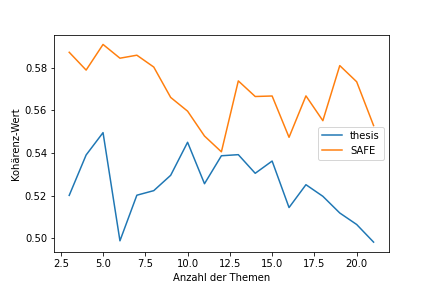
\includegraphics[width=\textwidth]{media/cs_PH_A01.png}
         \caption{PH\_01}
         \label{fig:lda-a01}
     \end{subfigure}
     \hfill
     \begin{subfigure}[b]{0.495\textwidth}
         \centering
         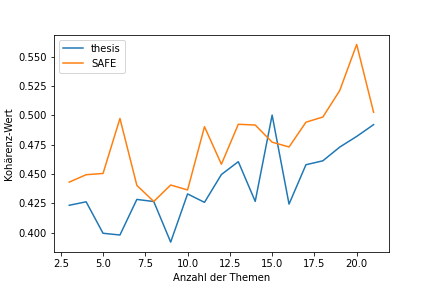
\includegraphics[width=\textwidth]{media/cs_PH_A02.png}
         \caption{PH\_02}
         \label{fig:lda-a02}
     \end{subfigure}
     \hfill
     \begin{subfigure}[b]{0.495\textwidth}
         \centering
         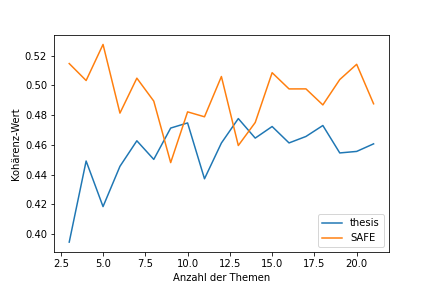
\includegraphics[width=\textwidth]{media/cs_PH_A03.png}
         \caption{PH\_03}
         \label{fig:lda-a03}
     \end{subfigure}
     \hfill
     \begin{subfigure}[b]{0.495\textwidth}
         \centering
         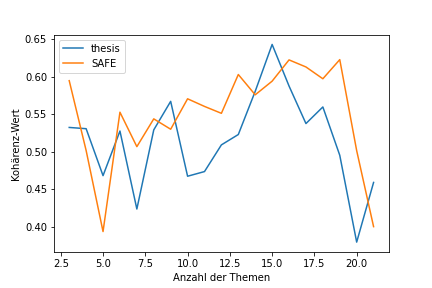
\includegraphics[width=\textwidth]{media/cs_PH_A04.png}
         \caption{PH\_04}
         \label{fig:lda-a04}
     \end{subfigure}
    \caption{Ergebnisse der Themenmodellierung: PH\_A01-04}
    \label{app:figs:tmtopiccoherence-external}
\end{figure}

\begin{sidewaysfigure}[!ht]
    \centering
    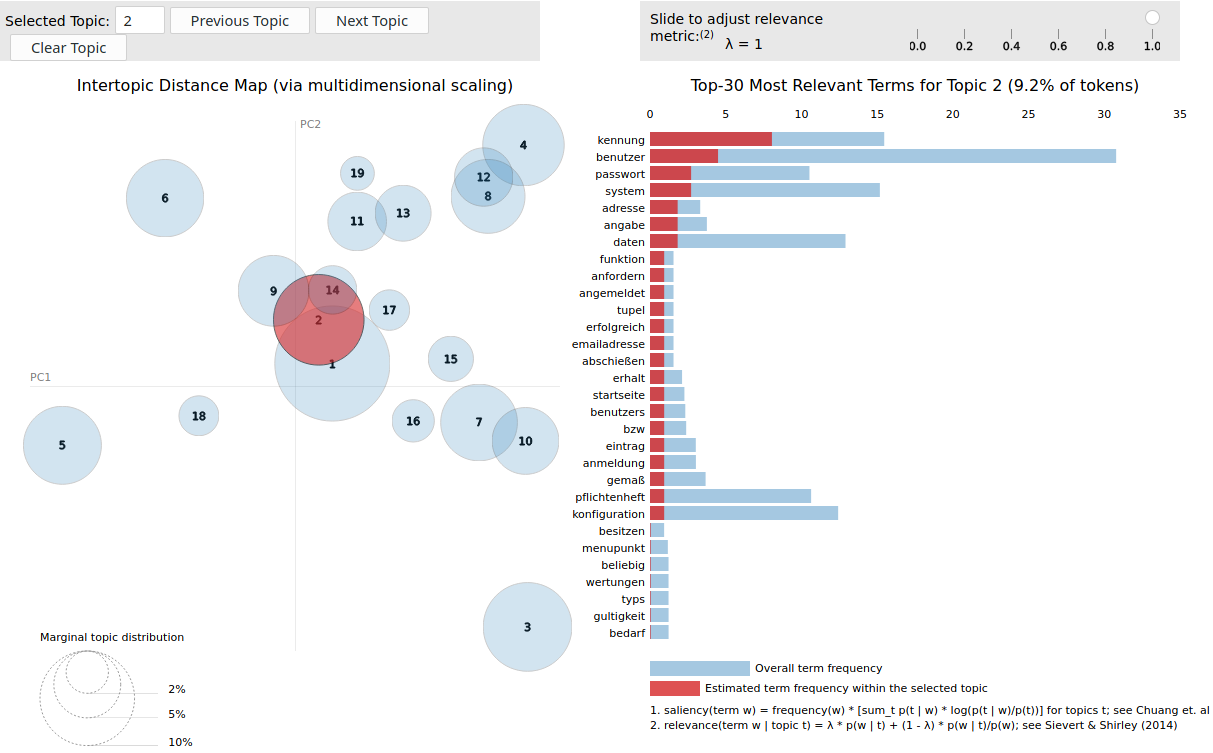
\includegraphics[width=\linewidth]{media/LDAVIZ_PH_A02.png}
    \caption{Visualisierte Themen des PH\_A04 mit pyLDAvis}
    \label{app:fig:lda_viz}
\end{sidewaysfigure}

\section{USB-Massenspeicher}

\vspace{0.5cm}

Auf dem beigelegten USB-Massenspeicher befinden sich:

\begin{itemize}
    \item Bachelorarbeit im PDF-Format
    \item Programmcode
    \begin{itemize}
        \item Jupyter Lab Projekt
        \item PyCharm Projekt
    \end{itemize}
\end{itemize}
